\section{More about Functions} \label{S:moreaboutfunctions}
\setcounter{previewactivity}{0}
%
%\begin{previewactivity}[A Function Defined by a Congruence] \label{PA:functioncongruence} \hfill \\
Write complete statements of Theorem~\ref{T:congtorem}  and  Corollary~\ref{C:congtorem}   from Section~\ref{S:cases}.
%\vskip10pt
%\noindent
%\textbf{Theorem~\ref{T:congtorem}} \emph{Let  $n \in \mathbb{N}$ and let  $a \in \mathbb{Z}$.  If  $a = nq + r\text{  and  }0 \leq r < n$ for some integers  $q$  and  $r$, then  
%$a \equiv r \pmod n$.}
%\vskip10pt

Theorem~\ref{T:congtorem} and Corollary~\ref{C:congtorem} state that an integer is congruent (mod $n$) to its remainder when it is divided by  $n$.  (Recall that we always mean the remainder guaranteed by the Division Algorithm, which is the least nonnegative remainder.)  Since this remainder is unique and since the only possible remainders for division by $n$  are  $0, 1, 2,  \ldots , n - 1$, we then know that each integer is congruent, modulo $n$, to precisely one of the integers $0,1,2, \ldots ,n - 1$.
%\vskip10pt
%\noindent
%\textbf{Corollary~\ref{C:congtorem}} \emph{If  $n \in \mathbb{N}$, then each integer is congruent, modulo n, to precisely one of the integers $0,1,2, \ldots ,n - 1$.}
%\vskip10pt
%
\begin{enumerate}
\item Define the set  $\mathbb{Z}_6 $ to be  $\mathbb{Z}_6  = \left\{ {0, 1, 2, 3, 4, 5} \right\}$.  For each  $x \in \mathbb{Z}_6 $, compute  $x^2  + 3$ and then determine the value of  $r$  in  $\mathbb{Z}_6 $ so that
\[
\left( {x^2  + 3} \right) \equiv r\pmod 6.
\]
For example,  $2^2  + 3 = 7$ and so  $\left( {2^2  + 3} \right) \equiv 1 \pmod 6$.  Organize your results in a table with one column for the value of $x$ and another column for the value of $r$, where $r \in \mathbb{Z}_6$ and $\left( {x^2  + 3} \right) \equiv r\pmod 6$. 
\label{PA:functioncongruence1}

\item Explain how your work in Part~(\ref{PA:functioncongruence1}) can be used to define a function from   $\mathbb{Z}_6 $
to  $\mathbb{Z}_6 $.

\end{enumerate}
\end{previewactivity}
\hbreak
%
%
\begin{previewactivity}[The Number of Diagonals of a Polygon] \label{PA:diagonals} \hfill \\
A \textbf{polygon}
\index{polygon}%
 is a closed plane figure formed by the joining of three or more straight lines. For example, a \textbf{triangle}
\index{triangle}%
 is a polygon that has three sides; a \textbf{quadrilateral}
\index{quadrilateral}%
 is a polygon that  has four sides and includes squares, rectangles, and parallelograms; a \textbf{pentagon}
\index{pentagon}%
 is a polygon that  has five sides; and an \textbf{octagon}
\index{octagon}%
 is a polygon that has eight sides. A \textbf{regular polygon}
\index{regular polygon}%
\index{polygon!regular}%
 is one that has equal-length sides and congruent interior angles.

A \textbf{diagonal of a polygon}
\index{diagonal}%
\index{polygon!diagonal}%
 is a line segment that connects two nonadjacent vertices of the polygon.  In this activity, we will assume that all polygons are convex polygons so that, except for the vertices, each diagonal lies inside the polygon.

\begin{enumerate}
\item How many diagonals does a triangle have?  How many diagonals does a square have?  How many diagonals does any quadrilateral have?

\item Let   $D = \mathbb{N} - \left\{ {1, 2} \right\}$.  Define   
$d\x D \to \mathbb{N} \cup \left\{ 0 \right\}$ so that   $d( n )$ is the number of diagonals of a  convex polygon with  $n$  sides.   Determine the values of $d(3)$, $d(4)$, $d(5)$, $d(6)$, $d(7)$, and $d(8)$.  Arrange the results in the form of a table of values for the function $d$.
\label{PA:diagonals2}
%Complete the following table, which shows the values of  $d\left( n \right)$ for selected values of  $n$.  
%
%\begin{center}
%\begin{tabular}{ c | c  c  c | c }
%  $n$   &  $d\left( n \right)$  &  &  $n$  &  $d\left( n \right)$ \\ \cline{1-2} \cline{4-5}
%   3    &                       &  &   6   &  \\ \cline{1-2} \cline{4-5}
%   4    &                       &  &   7   &  \\ \cline{1-2} \cline{4-5}
%   5    &                       &  &   8   &  \\ \cline{1-2} \cline{4-5}
%\end{tabular}
%\end{center}

\item Let  $f\x \mathbb{R} \to \mathbb{R}$  be defined by  
\[
f( x ) = \frac{{x\left( {x - 3} \right)}}{2}.
\]
Determine the values of $f(0)$, $f(1)$, $f(2)$, $f(3)$, $f(4)$, $f(5)$, $f(6)$, $f(7)$, 
$f(8)$, and $f(9)$.  Arrange the results in the form of a table of values for the function $f$\!.
\label{PA:diagonals3}%

%Complete the following table, which shows the values of  $f\left( x \right)$  for selected values of  $x$.  
%\begin{center}
%\begin{tabular}{ c | c  c  c | c }
%  $x$   &  $f\left( x \right)$  &  &  $x$  &  $f\left( x \right)$ \\ \cline{1-2} \cline{4-5}
%   0    &                       &  &   5   &  \\ \cline{1-2} \cline{4-5}
%   1    &                       &  &   6   &  \\ \cline{1-2} \cline{4-5}
%   2    &                       &  &   7   &  \\ \cline{1-2} \cline{4-5}
%   3    &                       &  &   8   &  \\ \cline{1-2} \cline{4-5}
%   4    &                       &  &   9   &  \\ \cline{1-2} \cline{4-5}
%\end{tabular}
%\end{center}

\item	What (if any) are the differences between the functions described in Parts~(\ref{PA:diagonals2}) and~(\ref{PA:diagonals3})?  Explain.

\end{enumerate}
\end{previewactivity}
\hbreak

\begin{previewactivity}[Derivatives] \label{PA:derivatives} \hfill \\
In calculus, we learned how to find the derivatives
\index{derivative}%
 of certain functions.  For example, if
\[
f( x ) = x^2( {\sin x} ),
\]
then we can use the product rule to obtain
\[
f'( x ) = 2x( {\sin x} ) + x^2( {\cos x} ).
\]
\begin{enumerate}
\item If possible, find the derivative of each of the following functions:
\begin{multicols}{2}
\begin{enumerate}
  \item $f( x ) = x^4  - 5x^3  + 3x - 7$

  \item $g( x ) = \cos ( {5x} )$

  \item $h( x ) = \dfrac{{\sin x}}{x}$
	
  \item $k( x ) = e^{ - x^2 } $

  \item $r( x ) = \left| x \right|$
\end{enumerate}
\end{multicols}

\item Is it possible to think of differentiation as a function?  Explain.  If so, what would be the domain of the function, what could be the codomain of the function, and what is the rule for computing the element of the codomain (output) that is associated with a given element of the domain (input)?

\end{enumerate}
\end{previewactivity}
\hbreak


\endinput

\begin{center}
\begin{tabular}[h]{| c | c |}
\hline
             &  $r \in \mathbb{Z}_6 $ where \\
   $x$       &  $\left( {x^2  + 3} \right) \equiv r \pmod 6$ \\ \hline
    0        &   \\ \hline
    1        &   \\ \hline
    2        &   \\ \hline
    3        &   \\ \hline
    4        &   \\ \hline
    5        &   \\ \hline
\end{tabular}
\end{center}

%\begin{previewactivity}[\textbf{Functions Defined by a Congruence}]\label{PA:function-congruence} \hfill

Before beginning this activity, review the statements of  Theorem~\ref{T:congtorem}  and  Corollary~\ref{C:congtorem}   from Section~\ref{S:cases}.

Theorem~\ref{T:congtorem} and Corollary~\ref{C:congtorem} state that an integer is congruent (mod $n$) to its remainder when it is divided by  $n$.  (Recall that we always mean the remainder guaranteed by the Division Algorithm, which is the least nonnegative remainder.)  Since this remainder is unique and since the only possible remainders for division by $n$  are  $0, 1, 2,  \ldots , n - 1$, we then know that each integer is congruent, modulo $n$, to precisely one of the integers $0,1,2, \ldots ,n - 1$.  So for each natural number 
$n$, we will define a new set $\Z_n$ as follows:
\[
\Z_n = \{ 0, 1, 2, \ldots , n - 1 \}.
\]
For example, $\Z_4 = \{0, 1, 2, 3 \}$ and $\Z_6 = \{ 0, 1, 2, 3, 4, 5 \}$.
\begin{enumerate}
\item For each  $x \in \Z_6 $, compute  $x^2  + 3$ and then determine the value of  $r$  in  
$\Z_6 $ so that
\[
\left( {x^2  + 3} \right) \equiv r\pmod 6.
\]
For example,  $2^2  + 3 = 7$, and since $\mod {7}{1}{6}$, we obtain   
$\left( {2^2  + 3} \right) \equiv 1 \pmod 6$.  Organize your results in a table with one column for the value of $x$ and another column for the value of $r$, where $r \in \mathbb{Z}_6$ and $\left( {x^2  + 3} \right) \equiv r\pmod 6$. 
\label{PA:functioncongruence1}

\item Explain how your work in Part~(\ref{PA:functioncongruence1}) can be used to define a function from   $\mathbb{Z}_6 $ to  $\mathbb{Z}_6 $. \label{PA:functioncongruence2}
\end{enumerate}
We will now describe a way to specify the outputs of this type of a function using a formula involving a congruence.  This will be illustrated with another example.  Define  
$g\x \Z_4  \to  \Z_4 $  by  $g( x ) = r$,  where  
$r \in \mathbb{Z}_4 $ and  $x^3  \equiv r \pmod 4$.  Then
\begin{align*}
g( 0 ) &= 0 	\text{\qquad since \qquad}   0^3  \equiv 0 \pmod 4 \\
g( 1 ) &= 1 	\text{\qquad since \qquad}   1^3  \equiv 1 \pmod 4 \\
g( 2 ) &= 0 	\text{\qquad since \qquad}   2^3  \equiv 0 \pmod 4 \\
g( 3 ) &= 3 	\text{\qquad since \qquad}   3^3  \equiv 3 \pmod 4.
\end{align*}
Note that this information about the outputs of this function could also be communicated by means of an arrow diagram or by means of a table of values.
The verbal description and the notation for the outputs of this function we have used are quite cumbersome.  So we will use a more concise notation.  Instead of writing,   
``$g\x \mathbb{Z}_4  \to \mathbb{Z}_4 $  by  $g( x ) = r$,  where  $r \in \mathbb{Z}_4 $ and 
$x^3  \equiv r \pmod 4$,'' we will write
\[
g\x \mathbb{Z}_4  \to \mathbb{Z}_4 \text{  by  }g( x ) = x^3 \pmod 4.
\]
\setcounter{oldenumi}{\theenumi}
\begin{enumerate} \setcounter{enumi}{\theoldenumi}
\item Define the function from Parts~(\ref{PA:functioncongruence1}) and~(\ref{PA:functioncongruence2}) in a manner similar to the way the function $g$ was defined.
\end{enumerate}
\end{previewactivity}
\hbreak

\endinput

In Section~\ref{S:introfunctions}, we have seen many examples of functions.  We have also seen various ways to represent functions and to convey information about them.  For example, we have seen that the rule for determining outputs of a function can be given by a formula, a graph, or a table of values.  We have also seen that sometimes it is more convenient to give a verbal description of the rule for a function.  In cases where the domain and codomain are small, finite sets, we used an arrow diagram to convey information about how inputs and outputs are associated without explicitly stating a rule.  In this section, we will study some types of functions, some of which we may not have encountered in previous mathematics courses.

\begin{previewactivity}[\textbf{The Number of Diagonals of a Polygon}] \label{PA:diagonals} \hfill \\
A \textbf{polygon}
\index{polygon}%
 is a closed plane figure formed by the joining of three or more straight lines. For example, a \textbf{triangle}
\index{triangle}%
 is a polygon that has three sides; a \textbf{quadrilateral}
\index{quadrilateral}%
 is a polygon that  has four sides and includes squares, rectangles, and parallelograms; a \textbf{pentagon}
\index{pentagon}%
 is a polygon that  has five sides; and an \textbf{octagon}
\index{octagon}%
 is a polygon that has eight sides. A \textbf{regular polygon}
\index{regular polygon}%
\index{polygon!regular}%
 is one that has equal-length sides and congruent interior angles.

A \textbf{diagonal of a polygon}
\index{diagonal}%
\index{polygon!diagonal}%
 is a line segment that connects two nonadjacent vertices of the polygon.  In this activity, we will assume that all polygons are \textbf{convex polygons} so that, except for the vertices, each diagonal lies inside the polygon.  For example, a triangle (3-sided polygon) has no diagonals and a rectangle has two diagonals.

\begin{enumerate}
\item How many diagonals does any quadrilateral (4-sided polygon) have?

\item Let   $D = \mathbb{N} - \left\{ {1, 2} \right\}$.  Define   
$d\x D \to \mathbb{N} \cup \left\{ 0 \right\}$ so that   $d( n )$ is the number of diagonals of a  convex polygon with  $n$  sides.   Determine the values of $d(3)$, $d(4)$, $d(5)$, $d(6)$, $d(7)$, and $d(8)$.  Arrange the results in the form of a table of values for the function $d$.
\label{PA:diagonals2}

\item Let  $f\x \mathbb{R} \to \mathbb{R}$  be defined by  
\[
f( x ) = \frac{{x\left( {x - 3} \right)}}{2}.
\]
Determine the values of $f(0)$, $f(1)$, $f(2)$, $f(3)$, $f(4)$, $f(5)$, $f(6)$, $f(7)$, 
$f(8)$, and $f(9)$.  Arrange the results in the form of a table of values for the function $f$\!.
\label{PA:diagonals3}%


\item	Compare the functions in Parts~(\ref{PA:diagonals2}) and~(\ref{PA:diagonals3}).  What are the similarities between the two functions and what are the differences?  Should these two functions be considered equal functions?  Explain.
\end{enumerate}
\end{previewactivity}
\hbreak


\endinput

\begin{previewactivity}[\textbf{Derivatives}] \label{PA:derivatives} \hfill \\
In calculus, we learned how to find the derivatives
\index{derivative}%
 of certain functions.  For example, if $f( x ) = x^2( {\sin x} )$, then we can use the product rule to obtain
\[
f'( x ) = 2x( {\sin x} ) + x^2( {\cos x} ).
\]
\begin{enumerate}
\item If possible, find the derivative of each of the following functions:
\begin{multicols}{2}
\begin{enumerate}
  \item $f( x ) = x^4  - 5x^3  + 3x - 7$

  \item $g( x ) = \cos ( {5x} )$

  \item $h( x ) = \dfrac{{\sin x}}{x}$
	
  \item $k( x ) = e^{ - x^2 } $

  \item $r( x ) = \left| x \right|$
\end{enumerate}
\end{multicols}

\item Is it possible to think of differentiation as a function?  Explain.  If so, what would be the domain of the function, what could be the codomain of the function, and what is the rule for computing the element of the codomain (output) that is associated with a given element of the domain (input)?

\end{enumerate}
\end{previewactivity}
\hbreak

\endinput

%
%In Section~\ref{S:introfunctions} and in the beginning activities for this section, we have seen many examples of functions.  Functions are everywhere in mathematics.  We have also seen various ways to represent functions and to convey information about them.  For example, we have seen that the rule for determining outputs of a function can be given by a formula, a graph, or a table of values.  We have also seen that sometimes it is more convenient to give a verbal description of the rule for a function.  In cases where the domain and codomain are small, finite sets, we used an arrow diagram to convey information about how inputs and outputs are associated without explicitly stating a rule.  In this section, we will study some types of functions that we may not have encountered in previous mathematics courses.


\subsection*{Functions Involving Congruences} \label{sub:functioncong}
Theorem~\ref{T:congtorem} and Corollary~\ref{C:congtorem} (see page~\pageref{T:congtorem}) state that an integer is congruent (mod $n$) to its remainder when it is divided by  $n$.  (Recall that we always mean the remainder guaranteed by the Division Algorithm, which is the least nonnegative remainder.)  Since this remainder is unique and since the only possible remainders for division by $n$  are  $0, 1, 2,  \ldots , n - 1$, we then know that each integer is congruent, modulo $n$, to precisely one of the integers $0,1,2, \ldots ,n - 1$.  So for each natural number 
$n$, we will define a new set $R_n$ as the set of remainders upon division by $n$.  So \label{page:R_n}
\[
R_n = \{ 0, 1, 2, \ldots , n - 1 \}.
\]
For example, $R_4 = \{0, 1, 2, 3 \}$ and $R_6 = \{ 0, 1, 2, 3, 4, 5 \}$.  We will now explore a method to define a function from $R_6$ to $R_6$.

For each  $x \in R_6 $, we can compute $x^2  + 3$ and then determine the value of  $r$  in  
$R_6 $ so that
\[
\left( {x^2  + 3} \right) \equiv r\pmod 6.
\]
Since $r$ must be in $R_6$, we must have $0 \leq r < 6$.  The results are shown in the following table.

\begin{table}[h]
\begin{center}
\begin{tabular}[t]{| c | c | c | c | c |} \cline{1-2} \cline{4-5}
   &  $r$ where  &  &  & $r$ where   \\
$x$ & $( {x^2  + 3} ) \equiv r( {\bmod 6} )$ & &  $x$ &  
$( {x^2  + 3} ) \equiv r( {\bmod 6} )$ \\ \cline{1-2} \cline{4-5} %\hline
0  &  3  &  & 3  &  0  \\ \cline{1-2} \cline{4-5}
1  &  4  &  & 4  &  1  \\ \cline{1-2} \cline{4-5}
2  &  1  &  & 5  &  4  \\ \cline{1-2} \cline{4-5}
\end{tabular}
\caption{Table of Values Defined by a Congruence}
\label{Ta:congruence}
\end{center}
\end{table}
The value of  $x$  in the first column can be thought of as the input for a function with the value of  $r$  in the second column as the corresponding output.  Each input produces exactly one output.  So we could write  
\begin{center}
$f:R_6  \to R_6 $  by  $f( x ) = r$ where  
$( {x^2  + 3} ) \equiv r  {\pmod 6} $.
\end{center}
This description and the notation for the outputs of this function are quite cumbersome.  So we will use a more concise notation.  We will, instead, write 
\begin{center}
Let  $f\x R_6  \to R_6 $ by   
$f( x ) = \left( {x^2  + 3} \right) \pmod 6$.
\end{center}
\hbreak

\begin{prog}[\textbf{Functions Defined by Congruences}] \label{pr:congfunctions} \hfill \\
We have   $R_5  = \left\{ {0, 1, 2, 3, 4} \right\}$. Define 
\begin{center} $f\x R_5  \to R_5$ by $f(x) = x^4 \pmod 5$, for each $x \in R_5$; 

$g\x R_5 \to R_5$ by $g(x) = x^5 \pmod 5$, for each $x \in R_5$.
\end{center}
\begin{enumerate}
\item Determine $f(0)$, $f(1)$, $f(2)$, $f(3)$, and $f(4)$ and represent the function $f$ with an arrow diagram.
\item Determine $g(0)$, $g(1)$, $g(2)$, $g(3)$, and $g(4)$ and represent the function $g$ with an arrow diagram.
\end{enumerate}
\end{prog}
\hbreak

\endinput

\subsection*{Equality of Functions}
The idea of equality of functions has been in the background of our discussion of functions, and it is now time to discuss it explicitly.  The preliminary work for this discussion was \typeu Activity~\ref*{PA:diagonals}, in which 
$D = \mathbb{N} - \left\{ {1, 2} \right\}$, and there were two functions:
\begin{itemize}
\item $d\x D \to \mathbb{N} \cup \left\{ 0 \right\}$, where  $d( n )$ is the number of diagonals of a convex polygon with  $n$  sides

\item $f\x \mathbb{R} \to \mathbb{R}$, where  
$f( x ) = \dfrac{{x\left( {x - 3} \right)}}{2}$, for each real number $x$.
\end{itemize}

In \typeu Activity~\ref*{PA:diagonals}, we saw that these two functions produced the same outputs for certain values of the input (independent variable).  For example, we can verify that
\begin{align*}
  d( 3 ) &= f( 3 ) = 0, \qquad &d( 4 ) = f( 4 ) = 2,\\ 
  d( 5 ) &= f( 5 ) = 5, \qquad \text{and }  &d( 6 ) = f( 6 ) = 9. \\ 
\end{align*}
Although the functions produce the same outputs for some inputs, these are two different functions.  For example, the outputs of the function  $f$  are determined  by a formula, and the outputs of the function  $d$  are determined by a verbal description.  This is not enough, however, to say that these are two different functions.  Based on the evidence from \typeu Activity~\ref*{PA:diagonals},  we might make the following conjecture:
\begin{center}
For  $n \geq 3$,  $d( n ) = \dfrac{{n\left( {n - 3} \right)}}{2}$.
\end{center}
Although we have not proved this statement, it is a true statement. (See Exercise~\ref{exer:sec62-6}.)  However, we know the function $d$ and the function $f$ are not the same function.  For example,
\begin{itemize}
\item $f( 0 ) = 0$,  but  0  is not in the domain of  $d$;

\item $f( \pi ) = \dfrac{{\pi \left( {\pi  - 3} \right)}}{2}$, but $\pi $ is not in the domain of  $d$.

\end{itemize}

We thus see the importance of considering the domain and codomain of each of the two functions in determining whether the two functions are equal or not.  This motivates the following definition. 
%
\begin{defbox}{functionequality}{Two functions  $f$  and  $g$  are \textbf{equal}
\index{equal functions}%
\index{function!equality}%
 provided that
\begin{itemize}
\item The domain of  $f$  equals the domain of  $g$.  That is, \\ 
$\text{dom}( f ) = \text{dom}( g )$.

\item The codomain of  $f$  equals the codomain of  $g$.  That is,  \\
$\text{codom}( f ) = \text{codom}( g )$.

\item For each  $x$  in the domain of  $f$  (which equals the domain of  $g$),  \\
$f( x ) = g( x )$.

\end{itemize}}
\end{defbox}
%
\begin{prog}[\textbf{Equality of Functions}] \label{pr:equalfunc} \hfill \\
Let  $A$  be a nonempty set.  The \textbf{identity function on the set}
\index{identity function}%
  $\boldsymbol{A}$, denoted by  $I_A $\label{sym:idfunc}, is the function  $I_A\x A \to A$ defined by  $I_A ( x ) = x$ for every  $x$  in  $A$.   That is, for the identity map, the output is always equal to the input.

For this progress check, we will use the functions $f$ and $g$ from Progress 
Check~\ref{pr:congfunctions}. The identity function on the set $R_5$ is 
\begin{center} 
$I_{R_5}:R_5  \to R_5$ by $I_{R_5}(x) = x \pmod 5$, for each $x \in R_5$.
\end{center}
Is the identity function on $R_5$ equal to either of the functions $f$ or $g$ from Progress 
Check~\ref{pr:congfunctions}?  Explain.
\end{prog}
\hbreak

\endinput

\subsection*{Mathematical Processes as Functions}
Certain mathematical processes can be thought of as functions.  In \typeu Activity~\ref*{PA:derivatives}, we reviewed how to find the derivatives of certain functions, and we considered whether or not we could think of this differentiation process as a function.  If we use a differentiable function as the input and consider the derivative of that function to be the output, then we have the makings of a function.  Computer algebra systems such as \emph{Maple} and \textit{Mathematica} have this derivative function as one of their predefined operators.  %Even some calculators now have a derivative function.  

Different computer algebra systems will have different syntax for entering functions and for the derivative function.   The first step will be to input a real function $f$.  This is usually done by entering a formula for $f(x)$, which is valid for all real numbers $x$ for which $f(x)$ is defined.  The next step is to apply the derivative function to the function $f$.  For purposes of illustration, we will use $D$ to represent this derivative function.  So this function will give $D(f) = f'$.

For example, if we enter
\[
f(x) = x^2 \sin (x) 
\]
for the function $f$, we will get
\begin{center}
$D(f) = f'$, where $f'(x) = 2x\sin \left( x \right) + x^2 \cos \left( x \right)$.
\end{center}

%Following is some \emph{Maple} code (using the Classic Worksheet version of \emph{Maple}) that can be used to find the derivative function of the function given by  $f( x ) = x^2( {\sin x} )$.  The lines that start with the \emph{Maple} prompt, $\left[ > \right.$, are the lines typed by the user.  The centered lines following these show the resulting \emph{Maple} output.  The first line defines the function  $f$\!, and the second line uses the derivative function  $D$  to produce the derivative of the function  $f$\!.
%\vskip6pt
%\noindent
%$\left[ > \right.$ \texttt{f := x} $\to$ \texttt{x}$\; \widehat{ }\; \texttt{2} *$ \texttt{sin(x)};
%
%%$\left[ > \right.$ f :$=$ x $\to$ x$\; \widehat{ }\; 2 *$ sin(x);
%\[
%f: = x \to x^2 \sin \left( x \right)
%\]
%$\left[ > \right.$ \texttt{f1 := D(f)};
%\[
%f1: = x \to 2x\sin \left( x \right) + x^2 \cos \left( x \right)
%\]
We must be careful when determining the domain for the derivative function since there are functions that are not differentiable.  To make things reasonably easy, we will let  $F$  be the set of all real functions that are differentiable and call this the domain of the derivative function  $D$.  We will use the set  $T$ of all real functions as the codomain.  So our function  $D$  is
\[
D\x F \to T  \text{ by } D( f ) = f'.
\]
%\hbreak
%\newpage
%
\begin{prog}[\textbf{Average of a Finite Set of Numbers}]\label{pr:average} \hfill \\
\index{average!of a finite set of numbers}%
Let $A = \left\{ a_1, a_2, \ldots, a_n \right\}$ be a finite set whose elements are the distinct real numbers $a_1, a_2, \ldots, a_n$.  We define the \textbf{average of the set $A$} to be the real number $\bar{A}$, where
\[
\bar{A} = \frac{a_1 + a_2 + \cdots + a_n}{n}.
\]
\begin{enumerate}
\item Find the average of $A = \left\{ 3, 7, -1, 5 \right\}$.
\item Find the average of $B = \left\{ 7, -2, 3.8, 4.2, 7.1 \right\}$.
\item Find the average of $C = \left\{ \sqrt{2}, \sqrt{3}, \pi - \sqrt{3} \right\}$.
\item Now let $\mathscr{F}( \R )$ be the set of all nonempty finite subsets of $\R$.  That is, a subset $A$ of $\R$ is in $\mathscr{F}( \R )$ if and only if $A$ contains only a finite number of elements.  Carefully explain how the process of finding the average of a finite subset of $\R$ can be thought of as a function.  In doing this, be sure to specify the domain of the function and the codomain of the function.
\end{enumerate}
\end{prog}
\hbreak

\endinput

\subsection*{Sequences as Functions}
A sequence can be considered to be an infinite list of objects that are indexed (subscripted) by the natural numbers (or some infinite subset of  $\mathbb{N} \cup \left\{ 0 \right\}$).  Using this idea, we often write a sequence in the following form:
\[
a_1 , a_2 ,  \ldots , a_n ,  \ldots .
\]
In order to shorten our notation, we will often use the notation  
$\left\langle {a_n } \right\rangle $
 to represent this sequence.  Sometimes a formula can be used to represent the terms of a sequence, and we might include this formula as the  $n$th  term in the list for a sequence such as in the following example:
\[
1, \frac{1}{2}, \frac{1}{3},  \ldots , \frac{1}{n},  \ldots .
\]
In this case, the  $n^\text{th}$ term of the sequence is  $\dfrac{1}{n}$.  If we know a formula for the  $n$th term, we often use this formula to represent the sequence.  For example, we might say
\begin{center}
Define the sequence  $\left\langle {a_n } \right\rangle $  by  $a_n  = \dfrac{1}{n}$  for each  $n \in \mathbb{N}$.
\end{center}
This shows that this sequence is a function with domain  $\mathbb{N}$.  If it is understood that the domain is $\N$, we could refer to this as the sequence $\left\langle \dfrac{1}{n} \right \rangle$. Given an element of the domain, we can consider  $a_n $ to be the output.  In this case, we have used subscript notation to indicate the output rather than the usual function notation.  We could just as easily write  
\[
a( n ) = \frac{1}{n} \text{ instead of } a_n  = \frac{1}{n}.  
\]
We make the following formal definition.
%
\begin{defbox}{sequence}{An (infinite) \textbf{sequence}
\index{sequence}%
 is a function whose domain is  $\mathbb{N}$ or some infinite subset of  $\mathbb{N} \cup \left\{ 0 \right\}$.}
\end{defbox}

\begin{prog}[\textbf{Sequences}] \label{pr:sequences} \hfill \\
Find the sixth and tenth terms of the following sequences, each of whose domain is $\N$:
\begin{enumerate}
\item $\dfrac{1}{3}, \dfrac{1}{6}, \dfrac{1}{9}, \dfrac{1}{12}, \ldots$
\item $\langle a_n \rangle$, where $a_n = \dfrac{1}{n^2}$ for each $n \in \N$
\item $\langle (-1)^n \rangle$
\end{enumerate}
\end{prog}
\hbreak

\endinput

\subsection*{Functions of Two Variables} \label{ss:functiontwovar}
In Section~\ref{S:cartesian}, we learned how to form the Cartesian product of two sets.  Recall that a Cartesian product of two sets is a set of ordered pairs.  For example, the set $\Z \times \Z$ is the set of all ordered pairs, where each coordinate of an ordered pair is an integer.  Since a Cartesian product is a set, it could be used as the domain or codomain of a function.  For example, we could use  $\Z \times \Z$ as the domain of a function as follows:
%
\begin{center}
Let $f\x \mathbb{Z} \times \mathbb{Z} \to \mathbb{Z}$ be defined by  
$f( {m, n} ) = 2m + n$.
\end{center}

\begin{itemize}
\item Technically, an element of  $\mathbb{Z} \times \mathbb{Z}$  is an ordered pair, and so we should write  $f( {( {m, n} )} )$ for the output of the function  $f$   when the input is  the ordered pair 
$\left( {m, n} \right)$.  However, the double parentheses seem unnecessary in this context and there should be no confusion if we write  $f( {m, n} )$ for the output of the function  $f$   when the input is  
$\left( {m, n} \right)$.  So, for example, we simply write
\begin{align*}
  f( {3, 2} )    &= 2 \cdot 3 + 2 = 8,\text{ and} \\ 
  f( { - 4, 5} ) &= 2 \cdot \left( { - 4} \right) + 5 =  - 3. \\ 
\end{align*} 
\item Since the domain of this function is $\Z \times \Z$ and each element of $\Z \times \Z$ is an ordered pair of integers, we frequently call this type of function a \textbf{function of two variables}.
\index{function!of two variables}%
\end{itemize}

Finding the preimages of an element of the codomain for the function $f$, $\mathbb{Z}$, usually involves solving an equation with two variables.  For example, to find the preimages of  $0 \in \mathbb{Z}$, we need to find all ordered pairs  $\left( {m, n} \right) \in \mathbb{Z} \times \mathbb{Z}$ such that 
$f( {m, n} ) = 0$.  This means that we must find all ordered pairs  $\left( {m, n} \right) \in \mathbb{Z} \times \mathbb{Z}$ such that
\[
2m + n = 0.
\]
Three such ordered pairs are  $\left( {0, 0} \right)$, $\left( {1,  - 2} \right)$, and  $\left( { - 1, 2} \right)$.  In fact, whenever we choose an integer value for  $m$, we can find a corresponding integer  $n$  such that  $2m + n = 0$.  This means that  0  has infinitely many preimages, and it may be difficult to specify the set of all of the preimages of 0 using the roster method.  One way that can be used to specify this set is to use set builder notation and say that the following set consists of all of the preimages of 0:
\[
\left\{ { {\left( {m, n} \right) \in \mathbb{Z} \times \mathbb{Z} } \mid 2m + n = 0} \right\} = \left\{ { {\left( {m, n} \right) \in \mathbb{Z} \times \mathbb{Z} } \mid n =  - 2m} \right\}\!.
\]
The second formulation for this set was obtained by solving the equation  
\linebreak $2m + n = 0$
for  $n$.
%\end{example}
\hbreak

\begin{prog}[\textbf{Working with a Function of Two Variables}] \label{pr:function-two} \hfill \\
Let $g\x \mathbb{Z} \times \mathbb{Z} \to \mathbb{Z}$ be defined by  
$g( {m, n} ) = m^2 - n$ for all $\left(m, n \right) \in \Z \times \Z$.

\begin{enumerate}
\item Determine $g(0, 3)$, $g(3,-2)$, $g(-3, -2)$, and $g(7, -1)$.
\item Determine the set of all preimages of the integer 0 for the function $g$.  Write your answer using set builder notation.
\item Determine the set of all preimages of the integer 5 for the function $g$.  Write your answer using set builder notation.
\end{enumerate}

\end{prog}
\hbreak

\endinput

\endinput



\subsection*{Examples of Functions Using Verbal Descriptions}
\begin{enumerate}
\item \textbf{The birthday function}
\index{birthday function}%
 from Preview Activity~\ref{PA:birthdayfunction}  from Section~\ref{S:introfunctions}.  
In this case,   $b$   is the function that assigns to each person his or her birthday (month and day).  The domain of the function  $b$  is the set of all people and the codomain of  $b$  is the set of all days in a leap year (i.e., January 1 through December 31, including February 29).

\item The function  \textbf{balance}  that assigns to each customer with a savings account at ManyBucksBank  the balance in that customer's savings account at the end of the business day on March 3, 2006.  The domain for this function would be the set of all savings account customers for the bank, and we could use the set of all rational numbers as the codomain.

\note  For a given function, the codomain does not have to be the same as the range.  In this case, it might be quite a hassle to determine the range.  The range would consist of all of the actual savings account balances of the customers of ManyBucksBank at the end of the business day on March 3, 2006.   We often have some freedom in selecting the codomain.  In this case, since the savings balances are monetary values given in dollars and cents, it seemed reasonable to use the set of rational numbers as the codomain.

\item The \textbf{sum of the divisors function}
\index{sum of divisors function}%
 introduced in Preview Activity~\ref{PA:sumofdivisors} from Section~\ref{S:introfunctions} and studied further in Progresss Check~\ref{pr:codomainandrange} is an example of a function that can be given by a formula, but the verbal description may be easier to understand and use.  

Recall that  $s\x \mathbb{N} \to \mathbb{N}$,  where for each  $n \in \mathbb{N}$,  
$s( n )$ is the sum of the distinct natural number divisors of  $n$.  This is a function that is studied and used in number theory, where a formula is determined for  $s\left( n \right)$
.  This formula can be written as
\[
s( n ) = \sum\limits_{d\left| n \right.} d .
\]
We do not have to worry about this notation in this text.  Basically, the formula says that  
$s( n )$ is the sum of all natural numbers  $d$,  where  $d$  divides  $n$.  Which formulation of  $s( n )$  is easier to understand?
\end{enumerate}
\hbreak
%

\begin{activity}[Integration as a Function] \label{A:integration} \hfill \\
In calculus, we learned that if  $f$  is real function that is continuous on the closed interval  $\left[ {a, b} \right]$, then the definite integral  $\int_a^b {f( x ) \, dx} $ is a real number.  In fact, one form of the \textbf{Fundamental Theorem of Calculus}
\index{Fundamental Theorem!of Calculus}%
 states that
\[
\int_a^b {f( x ) \, dx} = F( b ) - F( a ),
\]
where  $F$  is any antiderivative of  $f$, that is, where  $F \,' = f$\!.
%
\begin{enumerate}
\item Let  $\left[ {a, b} \right]$ be a closed interval of real numbers and let  
$C {\left[ {a, b} \right]} $ be the set of all real functions that are continuous on  
$\left[ {a, b} \right]$.  That is,
\[
C{\left[ {a, b} \right]}  = \left\{ {f\x \left[ {a, b} \right] \to \mathbb{R}  \mid f\text{ is continuous on }\left[ {a, b} \right]} \right\}.
\]
%
\begin{enumerate}
\item Explain how the definite integral   $\int_a^b {f( x ) \, dx} $  can be used to define a function  $I$  from  $C{\left[ {a, b} \right]} $ to  $\mathbb{R}$.

\item Let  $\left[ {a, b} \right] = \left[ {0, 2} \right]$.  Calculate  $I( f )$,
  where  $f( x ) = x^2  + 1$.

\item Let  $\left[ {a, b} \right] = \left[ {0, 2} \right]$.  Calculate  $I( g )$,
  where  $g( x ) = \sin ( {\pi x} )$.
\end{enumerate}
%
\end{enumerate}
%
In calculus, we also learned how to determine the indefinite integral  
$\int {f( x )} \;dx$ of a continuous function  $f$.

\begin{enumerate}
\setcounter{enumi}{1}
\item Let  $f( x ) = x^2  + 1$ and $g(x) = \cos( 2x )$. Determine  
$\int {f( x )} \;dx$ and $\int {g( x )} \;dx$.

\item Let  $f$  be a continuous function on the closed interval  $\left[ {0, 1} \right]$
  and let  $T$  be the set of all real functions.  Can the process of determining the indefinite integral of a continuous function be used to define a function from $C{\left[ {0, 1} \right]}$ to  $T$?  Explain.

\item Another form of the Fundamental Theorem of Calculus states that if  $f$  is continuous on the interval  $\left[ {a, b} \right]$ and if  
\[
g( x ) = \int_a^x {f( t ) \, dt}
\]
for each  $x$  in  $\left[ {a, b} \right]$, then  $g'\left( x \right) = f\left( x \right)$.  That is,  $g$  is an antiderivative of  $f$.  Explain how this theorem can be used to define a function from $C{\left[ {a,\;b} \right]} $ to  $T$\!,   where the output of the function is an antiderivative of the input.  (Recall that  $T$  is the set of all real functions.)

\end{enumerate}
\end{activity}
\hbreak
\endinput
%
%\subsection*{Some Standard Functions}
%The following are examples of functions that appear frequently in many areas of mathematics.
%
%\begin{enumerate}
%\item \textbf{The Identity Map} \hfill
%
%Let  $A$  be a nonempty set.  The \textbf{identity map on the set}
%\index{identity map}%
%  $\boldsymbol{A}$, denoted by  $I_A $ \label{sym:idfunc}, is the function  $I_A :A \to A$ defined by  $I_A \left( x \right) = x$ for every  $x$  in  $A$.   That is, for the identity map, the output is always equal to the input.
%
%\item \textbf{Constant Functions} \hfill
%
%Any function whose range consists of a single element is called a \textbf{constant function}.
%\index{constant function}%
%\index{function!constant}%
%  This term is used because for such a function, the output is always the same.  For example, let  $A$  and  $B$  be non-empty sets, and let  $b \in B$.  The function  $f:A \to B$ defined by  $f\left( x \right) = b$ for all  $x \in A$  is a constant function.
%
%\item \textbf{The Characteristic Function of a Set} \label{charfunction} \hfill
%
%Let  $A$  be a subset of some universal set  $U$.  The \textbf{characteristic function of the set}
%\index{characteristic function}%
%\index{function!characteristic}%
%  $\boldsymbol{A}$, denoted by  $\chi _A $, \label{sym:charfunc} is the function   
%$\chi _A :U \to \left\{ {0, 1} \right\}$ defined by
%\[
%\chi _A \left( x \right) = \left\{ \begin{gathered}
%  1\text{  if  }x \in A \hfill \\
%  0\text{  if  }x \notin A \hfill \\ 
%\end{gathered}  \right.
%\]
%The symbol  $\chi $  is the lower case letter  chi  in the Greek alphabet.  The characteristic function of  $A$  maps the elements of  $A$  to the number  1  and maps the elements of  the complement of $A$  to the element  0.  
%
%If  $A$  is a subset of  $\mathbb{R}$, then we can sketch a graph of its characteristic function.  For example,  if  $A = \left[ { - 1, 2} \right]$, then its graph would be the graph shown in Figure~\ref{fig:characteristicmap}.
%%\begin{figure}[h]
%%\begin{center}
%%\includegraphics{figpscharmap.bmp}
%%\caption{Graph of Characteristic Function of $A = \left[ { - 1, 2} \right]$} \label{fig:characteristicmap}
%%\end{center}
%%\end{figure}
%
%\begin{figure}[h]
%\begin{center}
%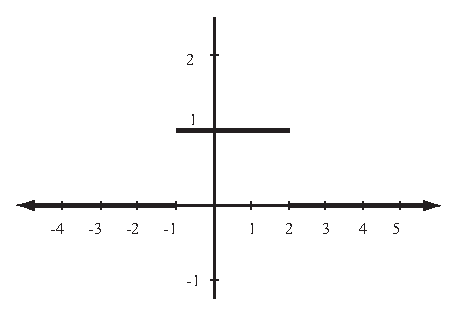
\includegraphics{figps-charfunction.eps}
%\caption{Graph of Characteristic Function of $A = \left[ { - 1, 2} \right]$} \label{fig:characteristicmap}
%\end{center}
%\end{figure}
%
%\item \textbf{Projection Functions}   \hfill
%
%Let  $A$  and  $B$  be two nonempty sets.  There are two \textbf{projection functions}
%\index{projection function}%
%\index{function!projection}%
% with domain  $A \times B$, the Cartesian product of  $A$  and  $B$.  One projection function will map an ordered pair to its first coordinate, and the other projection function will map the ordered pair to its second coordinate.   So we define  \label{sym:projfunc}
%\begin{list}{}
%\item $p_1 :A \times B \to A$ by $p_1 \left( {a, b} \right) = a$ for every  
%$\left( {a, b} \right) \in A \times B$; and 
%
%\item $p_2 :A \times B \to B$  by  $p_2 \left( {a, b} \right) = b$  for every  
%$\left( {a, b} \right) \in A \times B$. 
%\end{list}
%\end{enumerate}
%%
%\hbreak
%\subsection*{A Function as a Set of Ordered Pairs}
%\index{function!as set of ordered pairs}%
%
%When we graph a real function, we plot ordered pairs in the Cartesian plane where the first coordinate is the input of the function and the second coordinate is the output of the function.  For example, if  $g:\mathbb{R} \to \mathbb{R}$, then every point on the graph of  $g$  is an ordered pair  $\left( {x, y} \right)$ of real numbers where  $y = g\left( x \right)$.  This shows how we can generate ordered pairs from a function.  It happens that we can do this with any function.
%
%For example, let  
%\[
%A = \left\{ {1, 2, 3} \right\} \text{ and } B = \left\{ {a, b} \right\}.
%\]
%Define the function  $F:A \to B$ by  
%\[
%\begin{aligned}
%  F\left( 1 \right) &= a, \\ 
%  F\left( 2 \right) &= b,\text{ and} \\ 
%  F\left( 3 \right) &= b. \\ 
%\end{aligned}
%\]
%We can convert each of these to an ordered pair in  $A \times B$ by using the input as the first coordinate and the output as the second coordinate.  For example, 
%$F\left( 1 \right) = a$ is converted to $\left( 1, a \right)$, 
%$F\left( 2 \right) = b$ is converted to $\left( 2, b \right)$, and 
%$F\left( 3 \right) = b$ is converted to $\left( 3, b \right)$.  So, we can think of this function as a set of ordered pairs, which is a subset of  $A \times B$, and write
%\[
%F = \left\{ {\left( {1, a} \right), \left( {2, b} \right), \left( {3, b} \right)} \right\}.
%\]
%In fact, any function can be represented as a set of ordered pairs.  For example, if we have a real function, such as  $g:\mathbb{R} \to \mathbb{R}$  by  $g\left( x \right) = x^2  - 2$, then we can think of  $g$  as the following infinite subset of  $\mathbb{R} \times \mathbb{R}$:
%\[
%g = \left\{ { {\left( {x, y} \right) \in \mathbb{R} \times \mathbb{R}} \mid y = x^2  - 2} \right\}.
%\]
%If the context is clear, we usually simplify this to
%\[
%g = \left\{ {\left( {x, y} \right)} \mid y = x^2  - 2 \right\} \quad \text{ or } \quad
%g = \left\{ {\left( {x, x^2 - 2} \right)} \mid x \in \mathbb{R} \right\}.
%\]
%\hbreak
%%
%\begin{activity}[Defining a Function as a Set of Ordered Pairs] \label{A:funcasorderedparis} \hfill
%
%So far, we have started with a function and generated a set of ordered pairs that we can use to represent the function.  It is possible to reverse this process and first define a function as a special type of set of ordered pairs.  For example, if we started with  
%$A = \left\{ {1, 2, 3} \right\}$, $B = \left\{ {a, b} \right\}$, and defined
%\[
%F = \left\{ {\left( {1, a} \right), \left( {2, b} \right), \left( {3, b} \right)} \right\} \subseteq A \times B,
%\]
%then we could think of  $F$  as a function from  $A$  to  $B$  with  
%\[
%\begin{aligned}
%F\left( 1 \right) &= a, \\
%F\left( 2 \right) &= b, \text{ and} \\
%F\left( 3 \right) &= b. \\
%\end{aligned}
%\]
%\begin{enumerate}
%\item Could we use the following subset of  $A \times B$ to define a function from  $A$  to  $B$?  Explain.  \label{A:funcasorderedparis1}
%\[
%f = \left\{ {\left( {1, a} \right), \left( {2, a} \right), \left( {3, a} \right), \left( {1, b} \right)} \right\}
%\]
%
%\item Could we use the following subset of  $A \times B$ to define a function from  $A$  to  $B$?  Explain.   \label{A:funcasorderedparis2}
%\[
%g = \left\{ {\left( {1, a} \right), \left( {2, b} \right), \left( {3, a} \right)} \right\}
%\]
%
%\item Could we use the following subset of  $A \times B$
% to define a function from  $A$  to  $B$?  Explain.  \label{A:funcasorderedparis3}
%\[
%h = \left\{ {\left( {1, a} \right), \left( {2, b} \right)} \right\}
%\]
%
%\end{enumerate}
%
%In Section~\ref{S:introfunctions}, we defined a function  $f$   from a set  $A$  to a set  $B$  to be a rule that associates with every element  $x$  of the set  $A$  exactly one element of the set  $B$. 
%
%\begin{enumerate}
%\setcounter{enumi}{3}
%\item Carefully reformulate the definition of a function  $f$   from a set  $A$  to a set  $B$  to be a set of ordered pairs that is a subset of  $A \times B$  that has some clearly defined property or properties.  The examples in Parts~(\ref{A:funcasorderedparis1}) through~(\ref{A:funcasorderedparis3}) may be of help in specifying these properties.  
%
%This definition should be equivalent to the definition of a function given in Section~\ref{S:introfunctions}.  This means that a function as defined in Section~\ref{S:introfunctions} should produce a subset of  $A \times B$  with the specified properties, and a subset of  $A \times B$  with the specified properties could be used to define a function with the first coordinate as the input and the second coordinate as the output.
%
%\end{enumerate}
%
%\noindent
%\underline{Note}:  Many mathematicians believe that this ordered pair representation of a function is the most rigorous definition of a function.  It allows us to use set theory to work with and compare functions.  For example, equality of functions becomes a question of equality of sets.  Therefore, many textbooks will use the ordered pair representation of a function as the definition of a function.
%
%\end{activity}
%\hbreak








